% This is samplepaper.tex, a sample chapter demonstrating the
% LLNCS macro package for Springer Computer Science proceedings;
% Version 2.20 of 2017/10/04
%
\documentclass[runningheads]{llncs}
%
\usepackage{graphicx}
\usepackage{todonotes}
% Used for displaying a sample figure. If possible, figure files should
% be included in EPS format.
%
% If you use the hyperref package, please uncomment the following line
% to display URLs in blue roman font according to Springer's eBook style:
% \renewcommand\UrlFont{\color{blue}\rmfamily}

\begin{document}
%
\title{Thesis paper in Seminar Business Processes and the Internet of Things on Conformance Checking Using Activity and Trace Embeddings.}
%
%\titlerunning{Abbreviated paper title}
% If the paper title is too long for the running head, you can set
% an abbreviated paper title here
%
\author{Jan Kruska}
%
%\authorrunning{Pegoraro et al.}
% First names are abbreviated in the running head.
% If there are more than two authors, 'et al.' is used.
%
%\institute{Chair of Process and Data Science\\Department of Computer Science, RWTH Aachen, Aachen, Germany
%	\email{\{pegoraro,wvdaalst\}@pads.rwth-aachen.de}\\
%	\url{http://www.pads.rwth-aachen.de/}}
%
\maketitle              % typeset the header of the contribution
%
\begin{abstract}
\todo{Abstract}
%\keywords{First keyword  \and Second keyword \and Another keyword.}
\end{abstract}
%
%
%
\section{Planned structure}
The following list shall give a short overview of both the intended general structure of the seminar paper. In each section the main questions that should be answered by it are listed.
\begin{enumerate}
	\item Abstract
	\item Introduction
	\item Background
	\begin{enumerate}
		\item What is conformance checking, how is it useful and why would you do it, which methods are there, what are advantages and disadvantages of said methods.
		\item What is NLP (briefly), what are embeddings generally and word embeddings specifically, what are word2vec and doc2vec and how do they approach the NLP problems.
		\item What parallels are there between NLP and conformance checking
		\item If there are these parallels, how could such NLP mechanism be adapted (theoretically not practically) for conformance checking, what could the advantages be of such an approach, what could be disadvantages and/or problems that will need addressing.
	\end{enumerate}
	\item Method
	\begin{enumerate}
		\item How were word2vec and doc2vec adapted to conformance checking in the paper (I.e. practical adaption)
	\end{enumerate}
	\item Results
	\begin{enumerate}
		\item What are the results given in the paper
		\item What metrics were used to evaluate the performance of the approach presented in the paper, are they appropriate, are there other possible metrics, if so why was this one choses, what advantages or disadvantages do different metrics have.
		\item What are the results when using their code and reproducing the results (ideally the same)
	\end{enumerate}
	\item Outlook
	\begin{enumerate}
		\item What future work do the authors suggest
		\item What problems were encountered when trying to reproduce the results from the paper. Could they be reproduced completely, just in part or not at all. If so are there suggestions on how could these problems be mitigated.
	\end{enumerate}
\end{enumerate}
\section{First Section}
\subsection{A Subsection Sample}
Please note that the first paragraph of a section or subsection is
not indented. The first paragraph that follows a table, figure,
equation etc. does not need an indent, either.

Subsequent paragraphs, however, are indented.

\subsubsection{Sample Heading (Third Level)} Only two levels of
headings should be numbered. Lower level headings remain unnumbered;
they are formatted as run-in headings.

\paragraph{Sample Heading (Fourth Level)}
The contribution should contain no more than four levels of
headings. Table~\ref{tab1} gives a summary of all heading levels.

\begin{table}
\caption{Table captions should be placed above the
tables.}\label{tab1}
\begin{tabular}{|l|l|l|}
\hline
Heading level &  Example & Font size and style\\
\hline
Title (centered) &  {\Large\bfseries Lecture Notes} & 14 point, bold\\
1st-level heading &  {\large\bfseries 1 Introduction} & 12 point, bold\\
2nd-level heading & {\bfseries 2.1 Printing Area} & 10 point, bold\\
3rd-level heading & {\bfseries Run-in Heading in Bold.} Text follows & 10 point, bold\\
4th-level heading & {\itshape Lowest Level Heading.} Text follows & 10 point, italic\\
\hline
\end{tabular}
\end{table}


\noindent Displayed equations are centered and set on a separate
line.
\begin{equation}
x + y = z
\end{equation}
Please try to avoid rasterized images for line-art diagrams and
schemas. Whenever possible, use vector graphics instead (see
Fig.~\ref{fig1}).

\begin{figure}
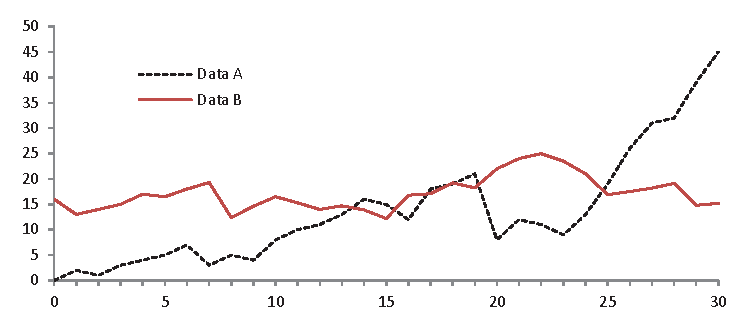
\includegraphics[width=\textwidth]{fig1.eps}
\caption{A figure caption is always placed below the illustration.
Please note that short captions are centered, while long ones are
justified by the macro package automatically.} \label{fig1}
\end{figure}

\begin{theorem}
This is a sample theorem. The run-in heading is set in bold, while
the following text appears in italics. Definitions, lemmas,
propositions, and corollaries are styled the same way.
\end{theorem}
%
% the environments 'definition', 'lemma', 'proposition', 'corollary',
% 'remark', and 'example' are defined in the LLNCS documentclass as well.
%
\begin{proof}
Proofs, examples, and remarks have the initial word in italics,
while the following text appears in normal font.
\end{proof}
For citations of references, we prefer the use of square brackets
and consecutive numbers. Citations using labels or the author/year
convention are also acceptable. The following bibliography provides
a sample reference list with entries for journal
articles~\cite{ref_article1}, an LNCS chapter~\cite{ref_lncs1}, a
book~\cite{ref_book1}, proceedings without editors~\cite{ref_proc1},
and a homepage~\cite{ref_url1}. Multiple citations are grouped
\cite{ref_article1,ref_lncs1,ref_book1},
\cite{ref_article1,ref_book1,ref_proc1,ref_url1}.
%
% ---- Bibliography ----
%
% BibTeX users should specify bibliography style 'splncs04'.
% References will then be sorted and formatted in the correct style.
%
\bibliographystyle{splncs04}
\bibliography{bibliography}
%
\end{document}
